\begin{frame}{反力のチェックサム(結果)}
 
% PrePoMaxにおいて、反力チェックサムを確認するには、以下設定する \\

 % TiKZを使った図形の描画 図2でA点を指し示す矢印
  \begin{textblock*}{0.95\linewidth}(-10pt,-5pt)
    \begin{figure}[htbp]
      \begin{center}
        \begin{tikzpicture}
	  \node [above right,minimum height=50pt, minimum width=420pt,align=left] at (0pt,0pt) {PrePoMaxにおいて、反力チェックサムを確認するには、以下設定する};
          \node[draw=blue,above right,minimum height=70pt,minimum width=110pt,align=left] at (20pt,-60pt)
		{ \scriptsize{合計された結果を見るには}\\
		  \scriptsize{XX-REACTION-FORCEの}\\
		  \scriptsize{TOATALFORCE-RF1のタグを}\\
		  \scriptsize{確認する}};
          \node[above right,minimum height=170pt,minimum width=260pt,align=left] at (130pt,-160pt) {
	    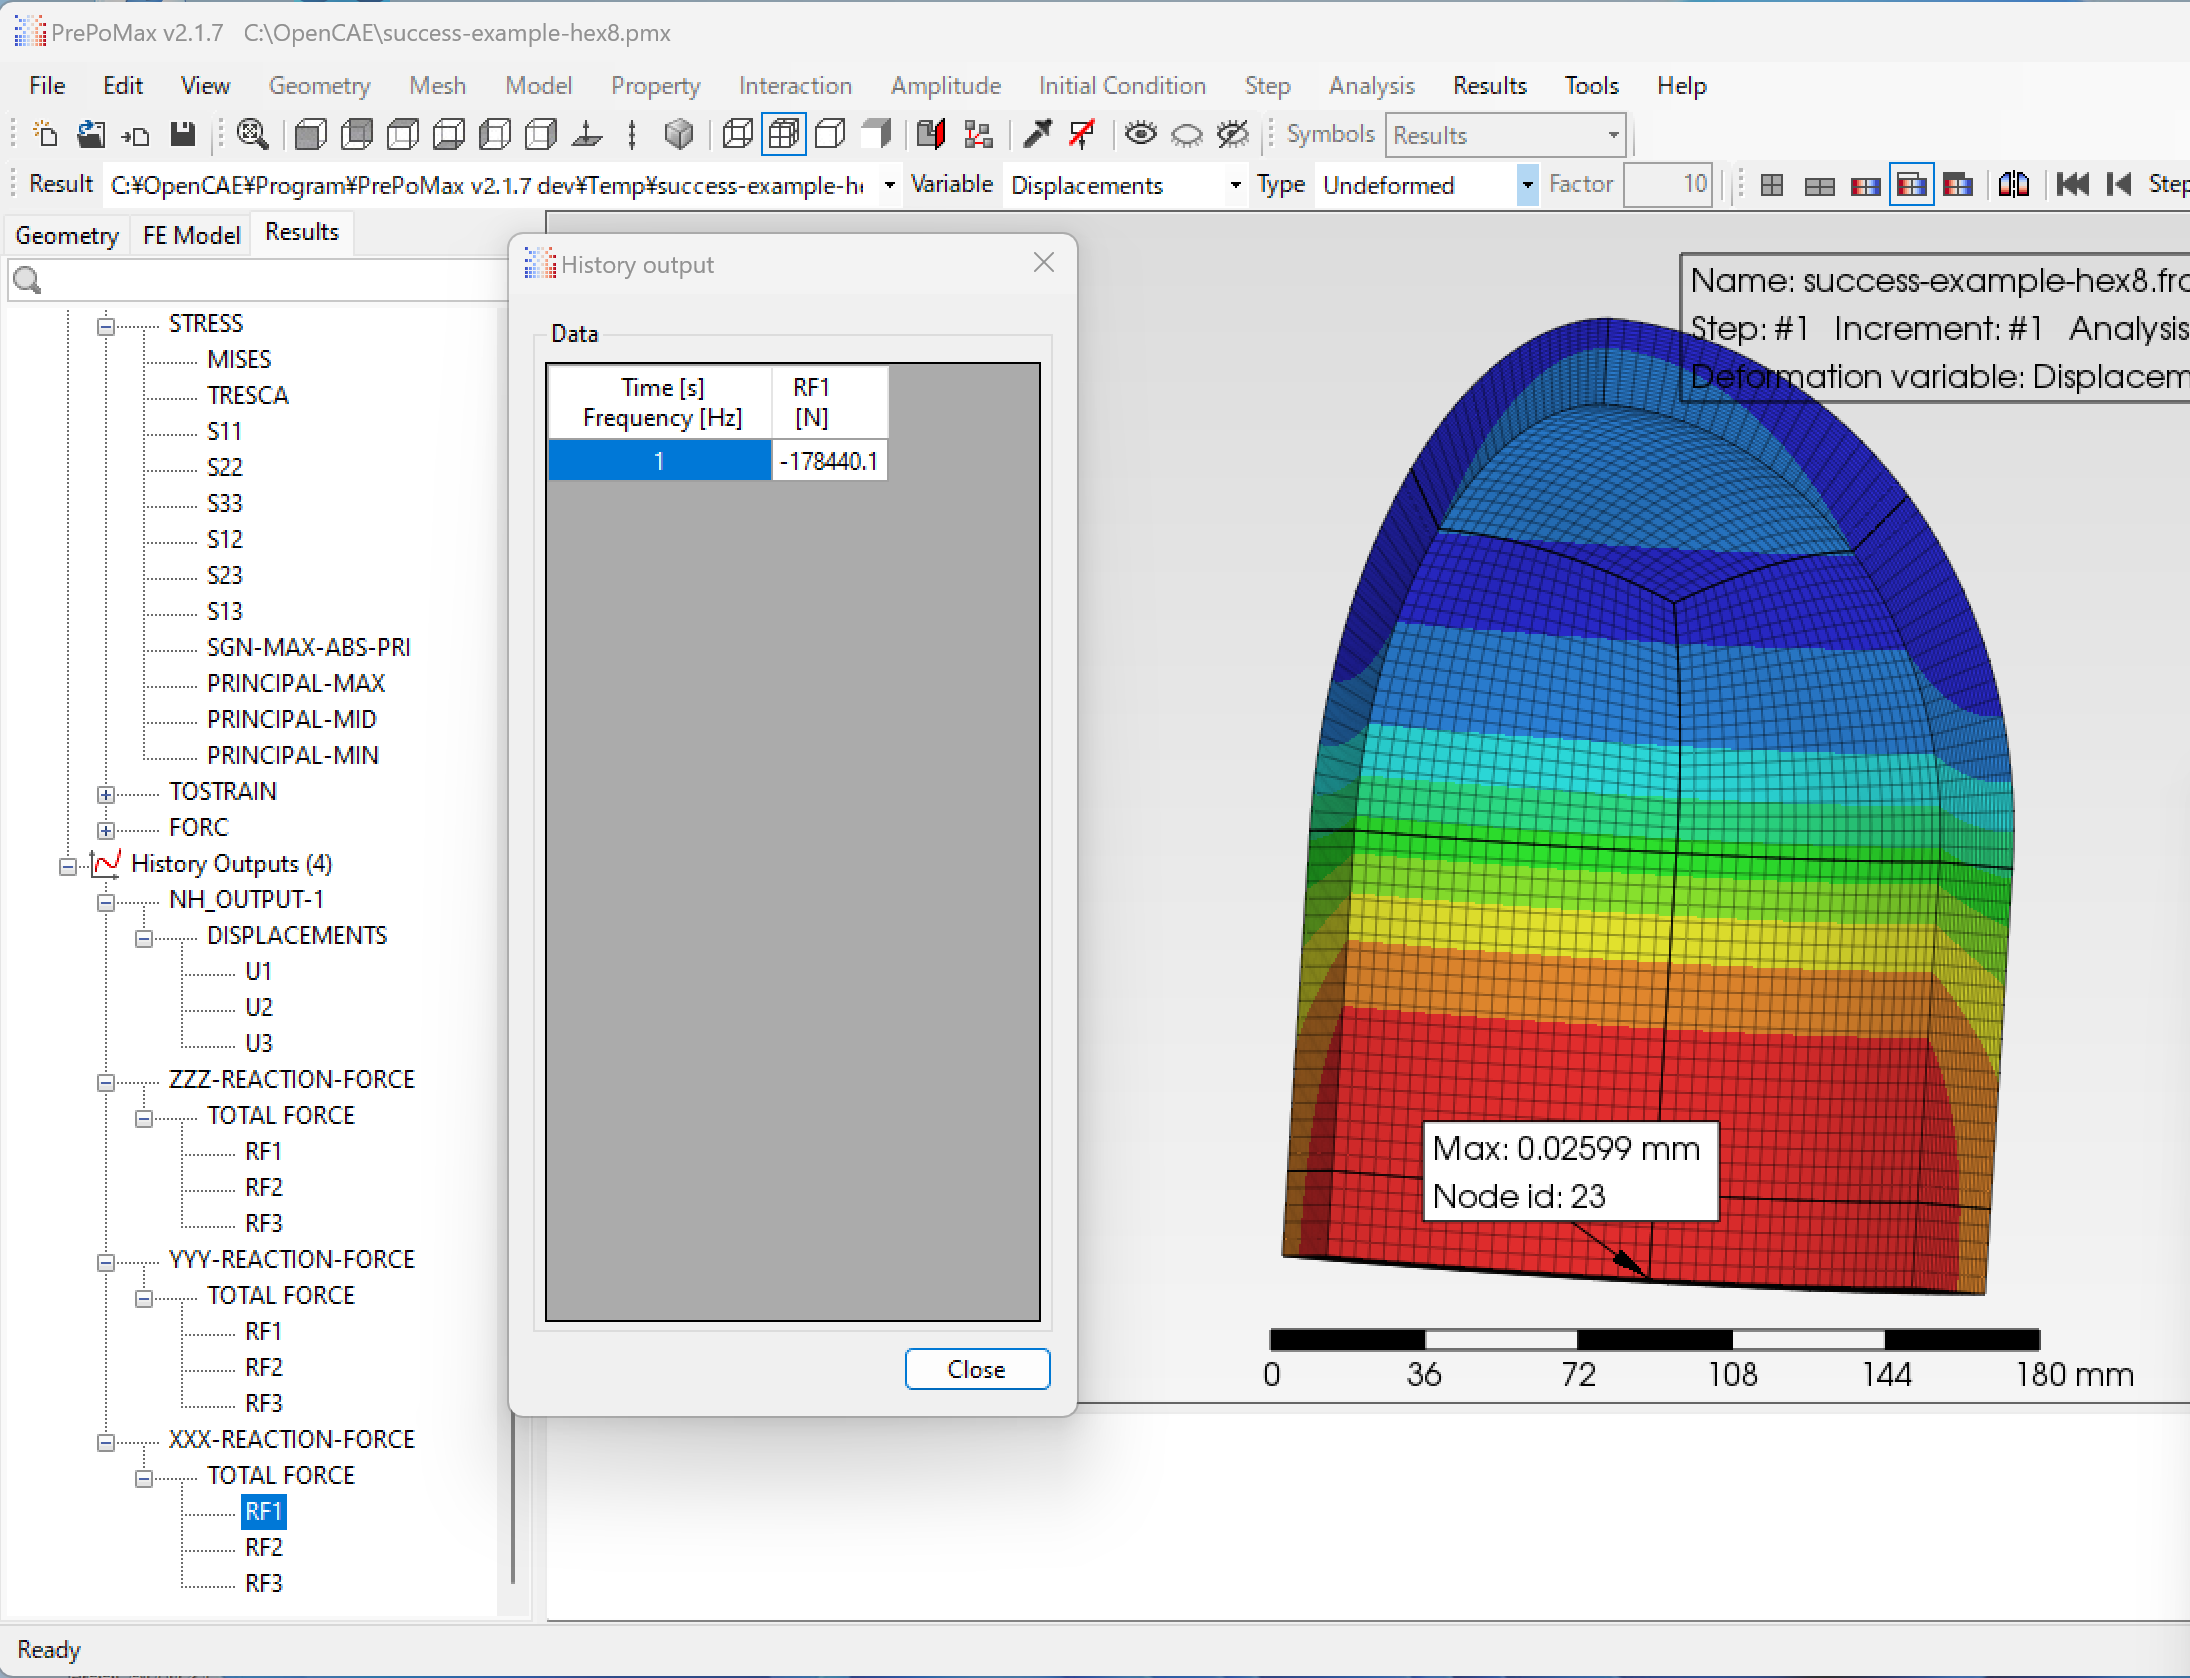
\includegraphics[keepaspectratio,scale=0.265] {images/screen02.png}};
          \draw[->, draw=cud_red, line width=1pt] (120pt,-60pt) -- (170pt,-140pt);
          \node[draw=blue,above right,minimum height=70pt,minimum width=100pt,align=left] at (20pt,-160pt)
		{ \scriptsize{この値がX方向から見た}\\
		  \scriptsize{受圧面の投影面積に面圧}\\
		  \scriptsize{をかけたものが}\\
		  \scriptsize{等しいか確認する}\\
		  \scriptsize{今回は誤差0.5\%}};
          \draw[->, draw=cud_red, line width=1pt] (120pt,-120pt) -- (227pt,-35pt);
        \end{tikzpicture}
        \caption{反力チェックサムの確認}
      \end{center}
    \end{figure}
  \end{textblock*}
\end{frame}
